\documentclass{standalone}
\usepackage{tikz}
\usetikzlibrary{positioning}

\begin{document}
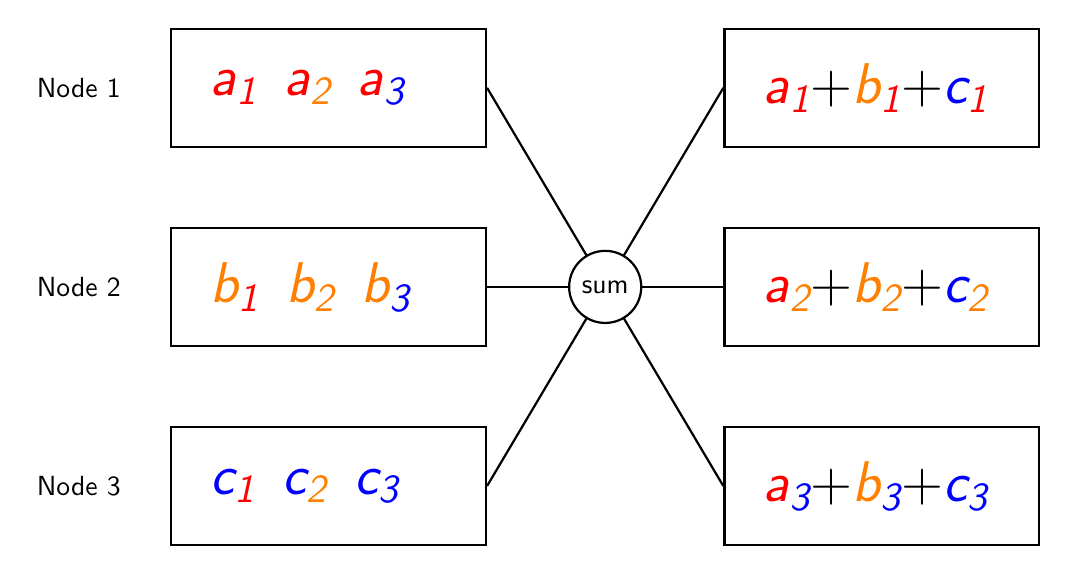
\begin{tikzpicture}[
    node distance=1cm,
    every node/.style={font=\sffamily},
    box/.style={draw, thick, minimum width=2cm, minimum height=1.5cm, align=center},
    longbox/.style={draw, thick, minimum width=4cm, minimum height=1.5cm, align=left, text width=3cm}
]

% 左侧节点
\node[longbox] (node1) {\itshape\huge{\color{red}a\textsubscript{\color{red}1}}\hspace{0.5em}{\color{red}a\textsubscript{\color{orange}2}}\hspace{0.5em}{\color{red}a\textsubscript{\color{blue}3}}};
\node[longbox, below=of node1] (node2) {\itshape\huge{\color{orange}b\textsubscript{\color{red}1}}\hspace{0.5em}{\color{orange}b\textsubscript{\color{orange}2}}\hspace{0.5em}{\color{orange}b\textsubscript{\color{blue}3}}};
\node[longbox, below=of node2] (node3) {\itshape\huge{\color{blue}c\textsubscript{\color{red}1}}\hspace{0.5em}{\color{blue}c\textsubscript{\color{orange}2}}\hspace{0.5em}{\color{blue}c\textsubscript{\color{blue}3}}};

% 左侧标签
\node[left=0.5cm of node1] {Node 1};
\node[left=0.5cm of node2] {Node 2};
\node[left=0.5cm of node3] {Node 3};

% 右侧长方形节点
\node[longbox, right=3cm of node1] (right1) {\huge{\itshape\color{red}a\textsubscript{\color{red}1}}+{\itshape\color{orange}b\textsubscript{\color{red}1}}+{\itshape\color{blue}c\textsubscript{\color{red}1}}};
\node[longbox, below=of right1] (right2) {\huge{\itshape\color{red}a\textsubscript{\color{orange}2}}+{\itshape\color{orange}b\textsubscript{\color{orange}2}}+{\itshape\color{blue}c\textsubscript{\color{orange}2}}};
\node[longbox, below=of right2] (right3) {\huge{\itshape\color{red}a\textsubscript{\color{blue}3}}+{\itshape\color{orange}b\textsubscript{\color{blue}3}}+{\itshape\color{blue}c\textsubscript{\color{blue}3}}};

% 连接线
% 从node1 (a) 出发的线
\draw[thick] (node1.east) -- (right3.west);
% 从node2 (b) 出发的线
\draw[thick] (node2.east) -- (right2.west);
% 从node3 (c) 出发的线
\draw[thick] (node3.east) -- (right1.west) node[midway,draw,fill=white,circle] {sum};

\end{tikzpicture}
\end{document}